\section{Python Problem}\label{sec:part5}

The script is written with Python 2.7. It uses cv2 to read images instead of scipy. Figure \ref{fig:ortho_proj} shows the projection of $x$ on different spaces $S_1, S_2, S_3, S_4,$ and $S_5$. Figure \ref{fig:tile_proj} and \ref{fig:tile_proj_color} show the projection of an image with resolution of 1024x768 (grayscale and color, respectively) on non-orthogonal tiles with $R=20$.

\begin{figure}[htbp]
	\centering
	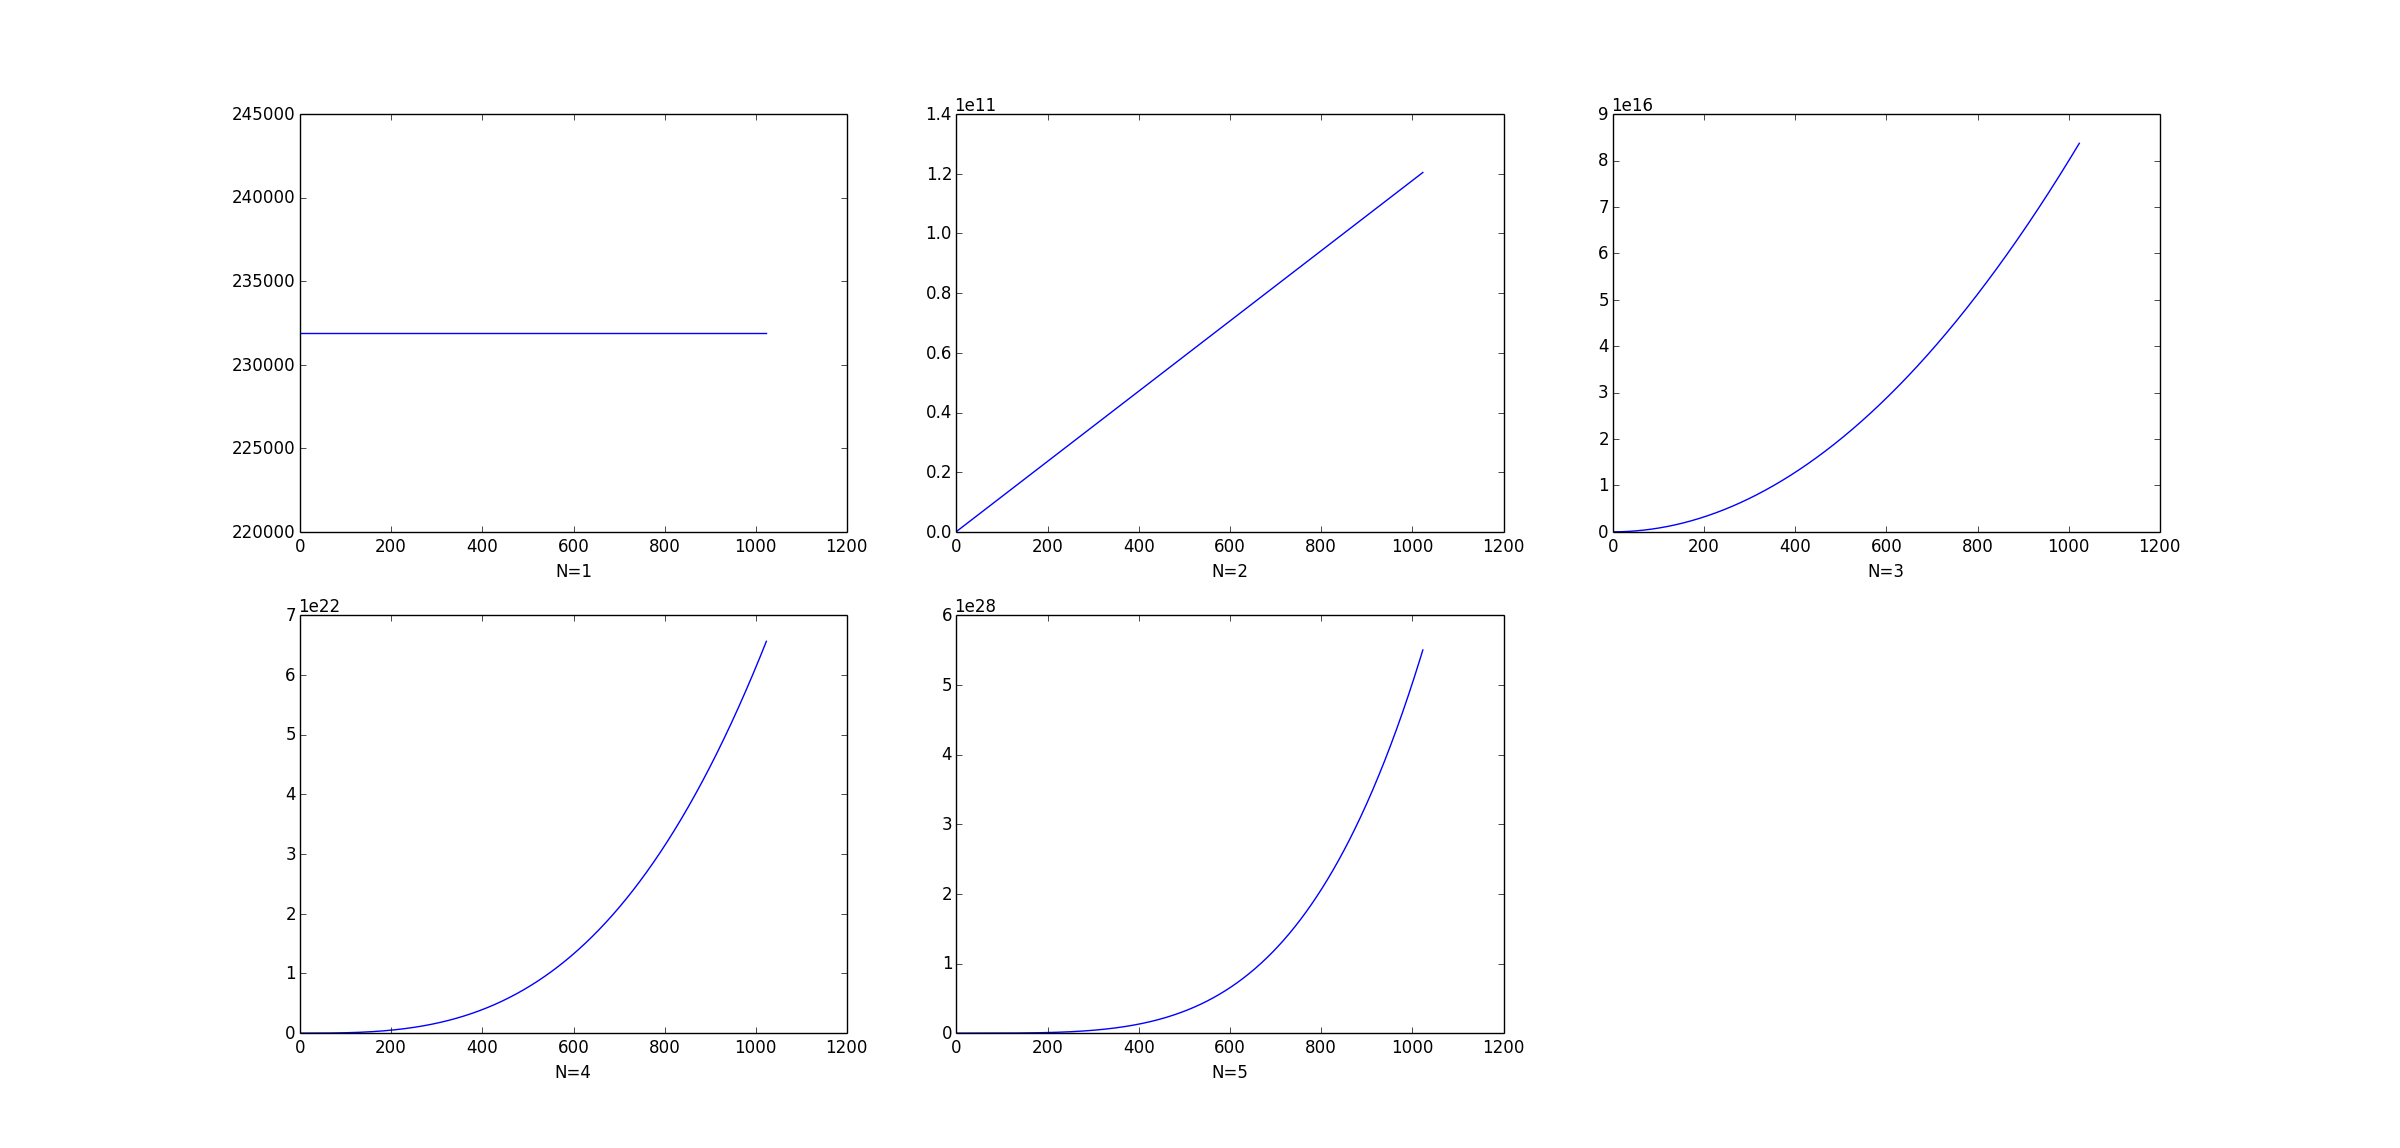
\includegraphics[width=\textwidth,trim={2in 0in 2in 1in},clip]{images/ortho_proj}
	\caption{Projecting $x$ on $S_1, S_2, S_3, S_4,$ and $S_5$.}\label{fig:ortho_proj}
\end{figure}

\begin{figure}[htbp]
	\centering
	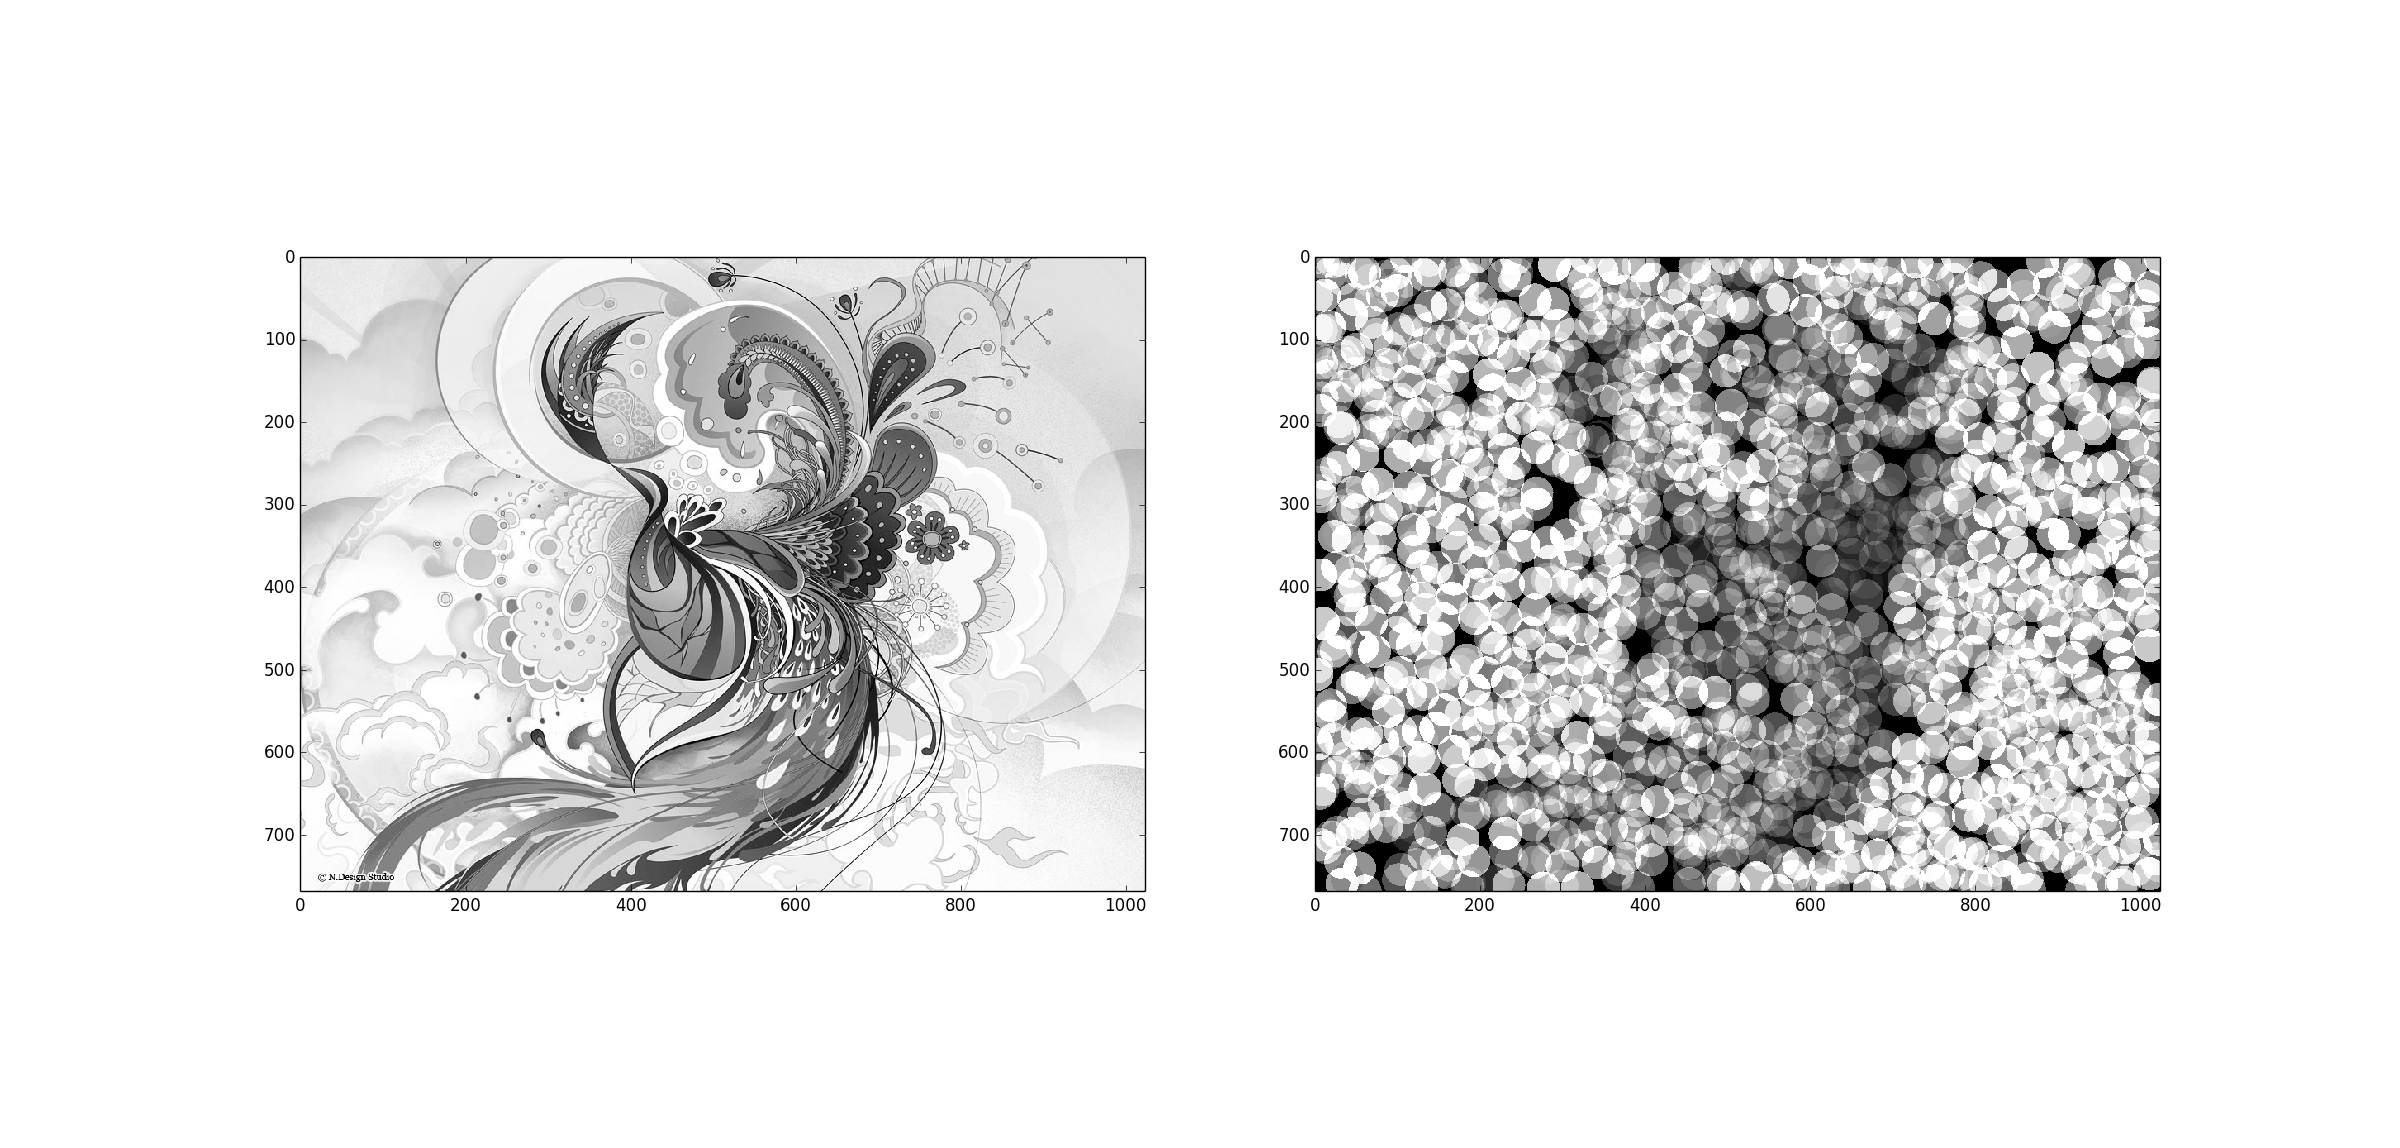
\includegraphics[width=\textwidth,trim={2.3in 1in 2.3in 1in},clip]{images/tile_proj}
	\caption{Projecting grayscale image on non-orthogonal tiles.}\label{fig:tile_proj}
\end{figure}

\begin{figure}[htbp]
	\centering
	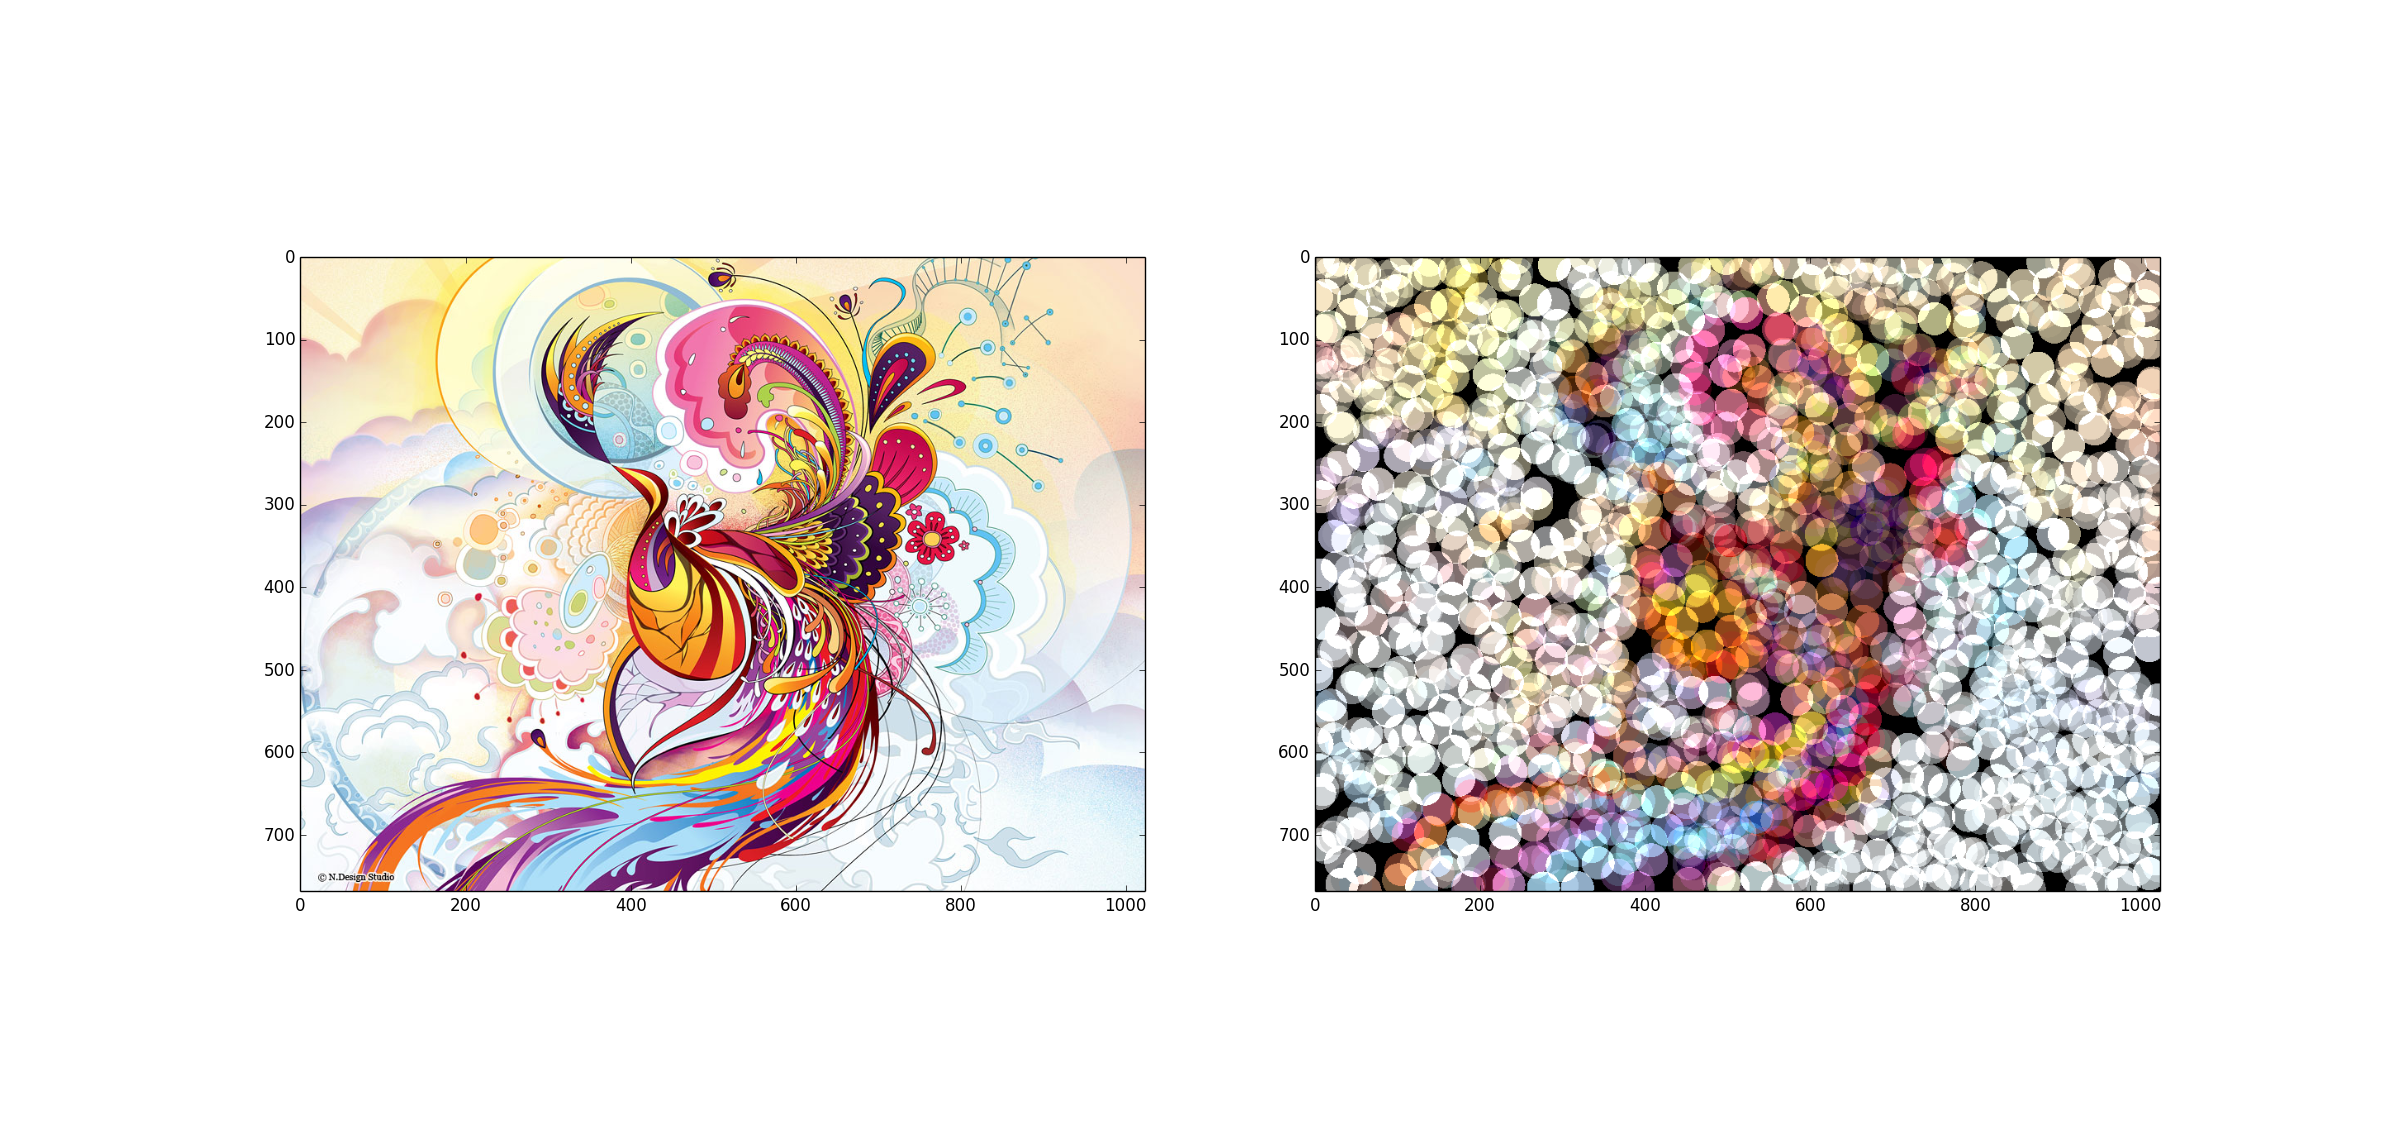
\includegraphics[width=\textwidth,trim={2.3in 1in 2.3in 1in},clip]{images/tile_proj_color}
	\caption{Projecting color image on non-orthogonal tiles.}\label{fig:tile_proj_color}
\end{figure}